% Options for packages loaded elsewhere
\PassOptionsToPackage{unicode}{hyperref}
\PassOptionsToPackage{hyphens}{url}
%
\documentclass[
]{article}
\usepackage{amsmath,amssymb}
\usepackage{lmodern}
\usepackage{iftex}
\ifPDFTeX
  \usepackage[T1]{fontenc}
  \usepackage[utf8]{inputenc}
  \usepackage{textcomp} % provide euro and other symbols
\else % if luatex or xetex
  \usepackage{unicode-math}
  \defaultfontfeatures{Scale=MatchLowercase}
  \defaultfontfeatures[\rmfamily]{Ligatures=TeX,Scale=1}
\fi
% Use upquote if available, for straight quotes in verbatim environments
\IfFileExists{upquote.sty}{\usepackage{upquote}}{}
\IfFileExists{microtype.sty}{% use microtype if available
  \usepackage[]{microtype}
  \UseMicrotypeSet[protrusion]{basicmath} % disable protrusion for tt fonts
}{}
\makeatletter
\@ifundefined{KOMAClassName}{% if non-KOMA class
  \IfFileExists{parskip.sty}{%
    \usepackage{parskip}
  }{% else
    \setlength{\parindent}{0pt}
    \setlength{\parskip}{6pt plus 2pt minus 1pt}}
}{% if KOMA class
  \KOMAoptions{parskip=half}}
\makeatother
\usepackage{xcolor}
\usepackage[margin=2.54cm]{geometry}
\usepackage{color}
\usepackage{fancyvrb}
\newcommand{\VerbBar}{|}
\newcommand{\VERB}{\Verb[commandchars=\\\{\}]}
\DefineVerbatimEnvironment{Highlighting}{Verbatim}{commandchars=\\\{\}}
% Add ',fontsize=\small' for more characters per line
\usepackage{framed}
\definecolor{shadecolor}{RGB}{248,248,248}
\newenvironment{Shaded}{\begin{snugshade}}{\end{snugshade}}
\newcommand{\AlertTok}[1]{\textcolor[rgb]{0.94,0.16,0.16}{#1}}
\newcommand{\AnnotationTok}[1]{\textcolor[rgb]{0.56,0.35,0.01}{\textbf{\textit{#1}}}}
\newcommand{\AttributeTok}[1]{\textcolor[rgb]{0.77,0.63,0.00}{#1}}
\newcommand{\BaseNTok}[1]{\textcolor[rgb]{0.00,0.00,0.81}{#1}}
\newcommand{\BuiltInTok}[1]{#1}
\newcommand{\CharTok}[1]{\textcolor[rgb]{0.31,0.60,0.02}{#1}}
\newcommand{\CommentTok}[1]{\textcolor[rgb]{0.56,0.35,0.01}{\textit{#1}}}
\newcommand{\CommentVarTok}[1]{\textcolor[rgb]{0.56,0.35,0.01}{\textbf{\textit{#1}}}}
\newcommand{\ConstantTok}[1]{\textcolor[rgb]{0.00,0.00,0.00}{#1}}
\newcommand{\ControlFlowTok}[1]{\textcolor[rgb]{0.13,0.29,0.53}{\textbf{#1}}}
\newcommand{\DataTypeTok}[1]{\textcolor[rgb]{0.13,0.29,0.53}{#1}}
\newcommand{\DecValTok}[1]{\textcolor[rgb]{0.00,0.00,0.81}{#1}}
\newcommand{\DocumentationTok}[1]{\textcolor[rgb]{0.56,0.35,0.01}{\textbf{\textit{#1}}}}
\newcommand{\ErrorTok}[1]{\textcolor[rgb]{0.64,0.00,0.00}{\textbf{#1}}}
\newcommand{\ExtensionTok}[1]{#1}
\newcommand{\FloatTok}[1]{\textcolor[rgb]{0.00,0.00,0.81}{#1}}
\newcommand{\FunctionTok}[1]{\textcolor[rgb]{0.00,0.00,0.00}{#1}}
\newcommand{\ImportTok}[1]{#1}
\newcommand{\InformationTok}[1]{\textcolor[rgb]{0.56,0.35,0.01}{\textbf{\textit{#1}}}}
\newcommand{\KeywordTok}[1]{\textcolor[rgb]{0.13,0.29,0.53}{\textbf{#1}}}
\newcommand{\NormalTok}[1]{#1}
\newcommand{\OperatorTok}[1]{\textcolor[rgb]{0.81,0.36,0.00}{\textbf{#1}}}
\newcommand{\OtherTok}[1]{\textcolor[rgb]{0.56,0.35,0.01}{#1}}
\newcommand{\PreprocessorTok}[1]{\textcolor[rgb]{0.56,0.35,0.01}{\textit{#1}}}
\newcommand{\RegionMarkerTok}[1]{#1}
\newcommand{\SpecialCharTok}[1]{\textcolor[rgb]{0.00,0.00,0.00}{#1}}
\newcommand{\SpecialStringTok}[1]{\textcolor[rgb]{0.31,0.60,0.02}{#1}}
\newcommand{\StringTok}[1]{\textcolor[rgb]{0.31,0.60,0.02}{#1}}
\newcommand{\VariableTok}[1]{\textcolor[rgb]{0.00,0.00,0.00}{#1}}
\newcommand{\VerbatimStringTok}[1]{\textcolor[rgb]{0.31,0.60,0.02}{#1}}
\newcommand{\WarningTok}[1]{\textcolor[rgb]{0.56,0.35,0.01}{\textbf{\textit{#1}}}}
\usepackage{graphicx}
\makeatletter
\def\maxwidth{\ifdim\Gin@nat@width>\linewidth\linewidth\else\Gin@nat@width\fi}
\def\maxheight{\ifdim\Gin@nat@height>\textheight\textheight\else\Gin@nat@height\fi}
\makeatother
% Scale images if necessary, so that they will not overflow the page
% margins by default, and it is still possible to overwrite the defaults
% using explicit options in \includegraphics[width, height, ...]{}
\setkeys{Gin}{width=\maxwidth,height=\maxheight,keepaspectratio}
% Set default figure placement to htbp
\makeatletter
\def\fps@figure{htbp}
\makeatother
\setlength{\emergencystretch}{3em} % prevent overfull lines
\providecommand{\tightlist}{%
  \setlength{\itemsep}{0pt}\setlength{\parskip}{0pt}}
\setcounter{secnumdepth}{-\maxdimen} % remove section numbering
\ifLuaTeX
  \usepackage{selnolig}  % disable illegal ligatures
\fi
\IfFileExists{bookmark.sty}{\usepackage{bookmark}}{\usepackage{hyperref}}
\IfFileExists{xurl.sty}{\usepackage{xurl}}{} % add URL line breaks if available
\urlstyle{same} % disable monospaced font for URLs
\hypersetup{
  pdftitle={Assignment 5: Data Visualization},
  pdfauthor={Emma Childs},
  hidelinks,
  pdfcreator={LaTeX via pandoc}}

\title{Assignment 5: Data Visualization}
\author{Emma Childs}
\date{Spring 2023}

\begin{document}
\maketitle

\hypertarget{overview}{%
\subsection{OVERVIEW}\label{overview}}

This exercise accompanies the lessons in Environmental Data Analytics on
Data Visualization

\hypertarget{directions}{%
\subsection{Directions}\label{directions}}

\begin{enumerate}
\def\labelenumi{\arabic{enumi}.}
\tightlist
\item
  Rename this file
  \texttt{\textless{}FirstLast\textgreater{}\_A05\_DataVisualization.Rmd}
  (replacing \texttt{\textless{}FirstLast\textgreater{}} with your first
  and last name).
\item
  Change ``Student Name'' on line 3 (above) with your name.
\item
  Work through the steps, \textbf{creating code and output} that fulfill
  each instruction.
\item
  Be sure your code is tidy; use line breaks to ensure your code fits in
  the knitted output.
\item
  Be sure to \textbf{answer the questions} in this assignment document.
\item
  When you have completed the assignment, \textbf{Knit} the text and
  code into a single PDF file.
\end{enumerate}

\begin{center}\rule{0.5\linewidth}{0.5pt}\end{center}

\hypertarget{set-up-your-session}{%
\subsection{Set up your session}\label{set-up-your-session}}

\begin{enumerate}
\def\labelenumi{\arabic{enumi}.}
\item
  Set up your session. Load the tidyverse, lubridate, here \& cowplot
  packages, and verify your home directory. Upload the NTL-LTER
  processed data files for nutrients and chemistry/physics for Peter and
  Paul Lakes (use the tidy
  \texttt{NTL-LTER\_Lake\_Chemistry\_Nutrients\_PeterPaul\_Processed.csv}
  version) and the processed data file for the Niwot Ridge litter
  dataset (use the
  \texttt{NEON\_NIWO\_Litter\_mass\_trap\_Processed.csv} version).
\item
  Make sure R is reading dates as date format; if not change the format
  to date.
\end{enumerate}

\begin{Shaded}
\begin{Highlighting}[]
\CommentTok{\#1 }
\FunctionTok{getwd}\NormalTok{()}
\end{Highlighting}
\end{Shaded}

\begin{verbatim}
## [1] "/home/guest/EDA-Spring2023"
\end{verbatim}

\begin{Shaded}
\begin{Highlighting}[]
\FunctionTok{install.packages}\NormalTok{(}\StringTok{"cowplot"}\NormalTok{)}
\end{Highlighting}
\end{Shaded}

\begin{verbatim}
## Installing package into '/home/guest/R/x86_64-pc-linux-gnu-library/4.2'
## (as 'lib' is unspecified)
\end{verbatim}

\begin{Shaded}
\begin{Highlighting}[]
\FunctionTok{library}\NormalTok{(tidyverse)}
\end{Highlighting}
\end{Shaded}

\begin{verbatim}
## -- Attaching core tidyverse packages ------------------------ tidyverse 2.0.0 --
## v dplyr     1.1.0     v readr     2.1.4
## v forcats   1.0.0     v stringr   1.5.0
## v ggplot2   3.4.1     v tibble    3.1.8
## v lubridate 1.9.2     v tidyr     1.3.0
## v purrr     1.0.1
\end{verbatim}

\begin{verbatim}
## -- Conflicts ------------------------------------------ tidyverse_conflicts() --
## x dplyr::filter() masks stats::filter()
## x dplyr::lag()    masks stats::lag()
## i Use the ]8;;http://conflicted.r-lib.org/conflicted package]8;; to force all conflicts to become errors
\end{verbatim}

\begin{Shaded}
\begin{Highlighting}[]
\FunctionTok{library}\NormalTok{(lubridate)}
\FunctionTok{library}\NormalTok{(here)}
\end{Highlighting}
\end{Shaded}

\begin{verbatim}
## here() starts at /home/guest/EDA-Spring2023
\end{verbatim}

\begin{Shaded}
\begin{Highlighting}[]
\FunctionTok{library}\NormalTok{(cowplot)}
\end{Highlighting}
\end{Shaded}

\begin{verbatim}
## 
## Attaching package: 'cowplot'
## 
## The following object is masked from 'package:lubridate':
## 
##     stamp
\end{verbatim}

\begin{Shaded}
\begin{Highlighting}[]
\CommentTok{\#installing and loading packages }

\NormalTok{NTL.Chem.Nutrients.PeterPaul }\OtherTok{\textless{}{-}} \FunctionTok{read.csv}\NormalTok{(}\AttributeTok{file=}\FunctionTok{here}\NormalTok{(}\StringTok{"./Data/Processed\_KEY/NTL{-}LTER\_Lake\_Chemistry\_Nutrients\_PeterPaul\_Processed.csv"}\NormalTok{), }\AttributeTok{stringsAsFactors =} \ConstantTok{TRUE}\NormalTok{)}
\NormalTok{NEON.litter }\OtherTok{\textless{}{-}} \FunctionTok{read.csv}\NormalTok{(}\AttributeTok{file=}\FunctionTok{here}\NormalTok{(}\StringTok{"./Data/Processed\_KEY/NEON\_NIWO\_Litter\_mass\_trap\_Processed.csv"}\NormalTok{), }\AttributeTok{stringsAsFactors =} \ConstantTok{TRUE}\NormalTok{)}
\CommentTok{\#reading in files}

\CommentTok{\#2 }
\NormalTok{NEON.litter}\SpecialCharTok{$}\NormalTok{collectDate }\OtherTok{\textless{}{-}} \FunctionTok{ymd}\NormalTok{(NEON.litter}\SpecialCharTok{$}\NormalTok{collectDate)}

\NormalTok{NTL.Chem.Nutrients.PeterPaul}\SpecialCharTok{$}\NormalTok{sampledate }\OtherTok{\textless{}{-}} \FunctionTok{ymd}\NormalTok{(NTL.Chem.Nutrients.PeterPaul}\SpecialCharTok{$}\NormalTok{sampledate)}
\CommentTok{\#Used \textquotesingle{}lubridate\textquotesingle{} to make sure dates are being read as date formats}
\end{Highlighting}
\end{Shaded}

\hypertarget{define-your-theme}{%
\subsection{Define your theme}\label{define-your-theme}}

\begin{enumerate}
\def\labelenumi{\arabic{enumi}.}
\setcounter{enumi}{2}
\tightlist
\item
  Build a theme and set it as your default theme. Customize the look of
  at least two of the following:
\end{enumerate}

\begin{itemize}
\tightlist
\item
  Plot background
\item
  Plot title
\item
  Axis labels
\item
  Axis ticks/gridlines
\item
  Legend
\end{itemize}

\begin{Shaded}
\begin{Highlighting}[]
\CommentTok{\#3}
\NormalTok{my\_theme }\OtherTok{\textless{}{-}} \FunctionTok{theme\_classic}\NormalTok{(}\AttributeTok{base\_size =} \DecValTok{12}\NormalTok{) }\SpecialCharTok{+} 
  \FunctionTok{theme}\NormalTok{(}
    \AttributeTok{plot.background =} \FunctionTok{element\_rect}\NormalTok{(}
      \AttributeTok{color =} \StringTok{\textquotesingle{}black\textquotesingle{}}\NormalTok{,}
      \AttributeTok{fill =} \StringTok{\textquotesingle{}lemonchiffon\textquotesingle{}}
\NormalTok{    ),}
    \AttributeTok{line =} \FunctionTok{element\_line}\NormalTok{(}
      \AttributeTok{color=}\StringTok{\textquotesingle{}purple\textquotesingle{}}\NormalTok{,}
      \AttributeTok{linewidth =}\DecValTok{2}
\NormalTok{    ),}
    \AttributeTok{legend.background =} \FunctionTok{element\_rect}\NormalTok{(}
      \AttributeTok{color=}\StringTok{\textquotesingle{}grey\textquotesingle{}}\NormalTok{,}
      \AttributeTok{fill =} \StringTok{\textquotesingle{}white\textquotesingle{}}
\NormalTok{    ),}
    \AttributeTok{legend.title =} \FunctionTok{element\_text}\NormalTok{(}
      \AttributeTok{color=}\StringTok{\textquotesingle{}black\textquotesingle{}}
\NormalTok{        ))}
    \FunctionTok{theme\_set}\NormalTok{(my\_theme)}
    
    \CommentTok{\#defining and setting custom theme after playing around with colors}
\end{Highlighting}
\end{Shaded}

\hypertarget{create-graphs}{%
\subsection{Create graphs}\label{create-graphs}}

For numbers 4-7, create ggplot graphs and adjust aesthetics to follow
best practices for data visualization. Ensure your theme, color
palettes, axes, and additional aesthetics are edited accordingly.

\begin{enumerate}
\def\labelenumi{\arabic{enumi}.}
\setcounter{enumi}{3}
\tightlist
\item
  {[}NTL-LTER{]} Plot total phosphorus (\texttt{tp\_ug}) by phosphate
  (\texttt{po4}), with separate aesthetics for Peter and Paul lakes. Add
  a line of best fit and color it black. Adjust your axes to hide
  extreme values (hint: change the limits using \texttt{xlim()} and/or
  \texttt{ylim()}).
\end{enumerate}

\begin{Shaded}
\begin{Highlighting}[]
\CommentTok{\#4 }
\NormalTok{NTL.LTER }\OtherTok{\textless{}{-}}\NormalTok{ NTL.Chem.Nutrients.PeterPaul }\SpecialCharTok{\%\textgreater{}\%}
  \FunctionTok{ggplot}\NormalTok{(}
    \FunctionTok{aes}\NormalTok{(}\AttributeTok{x=}\NormalTok{po4,}
      \AttributeTok{y=}\NormalTok{tp\_ug,}
      \AttributeTok{color=}\NormalTok{lakename)}
\NormalTok{    ) }\SpecialCharTok{+} 
  \FunctionTok{geom\_point}\NormalTok{(}\AttributeTok{size=}\FloatTok{0.5}\NormalTok{, }\AttributeTok{alpha=}\FloatTok{0.5}\NormalTok{) }\SpecialCharTok{+}
    \FunctionTok{labs}\NormalTok{(}
      \AttributeTok{title =} \StringTok{"Phosphorus and Phosphate Levels for Peter \& Paul Lakes"}\NormalTok{,}
      \AttributeTok{x=}\StringTok{"Phosphate (po4)"}\NormalTok{,}
      \AttributeTok{y=}\StringTok{"Phosphorus (ug)"}\NormalTok{, }
      \AttributeTok{color=}\StringTok{"Lakename"}
\NormalTok{    ) }\SpecialCharTok{+}
  \FunctionTok{geom\_smooth}\NormalTok{(}
    \AttributeTok{method =} \StringTok{\textquotesingle{}lm\textquotesingle{}}\NormalTok{,}
    \AttributeTok{se =} \ConstantTok{FALSE}\NormalTok{,}
    \AttributeTok{color =} \StringTok{\textquotesingle{}black\textquotesingle{}}\NormalTok{) }\SpecialCharTok{+}
    \FunctionTok{xlim}\NormalTok{(}\DecValTok{0}\NormalTok{,}\DecValTok{50}\NormalTok{)}

\FunctionTok{print}\NormalTok{(NTL.LTER)}
\end{Highlighting}
\end{Shaded}

\begin{verbatim}
## `geom_smooth()` using formula = 'y ~ x'
\end{verbatim}

\begin{verbatim}
## Warning: Removed 21947 rows containing non-finite values (`stat_smooth()`).
\end{verbatim}

\begin{verbatim}
## Warning: Removed 21947 rows containing missing values (`geom_point()`).
\end{verbatim}

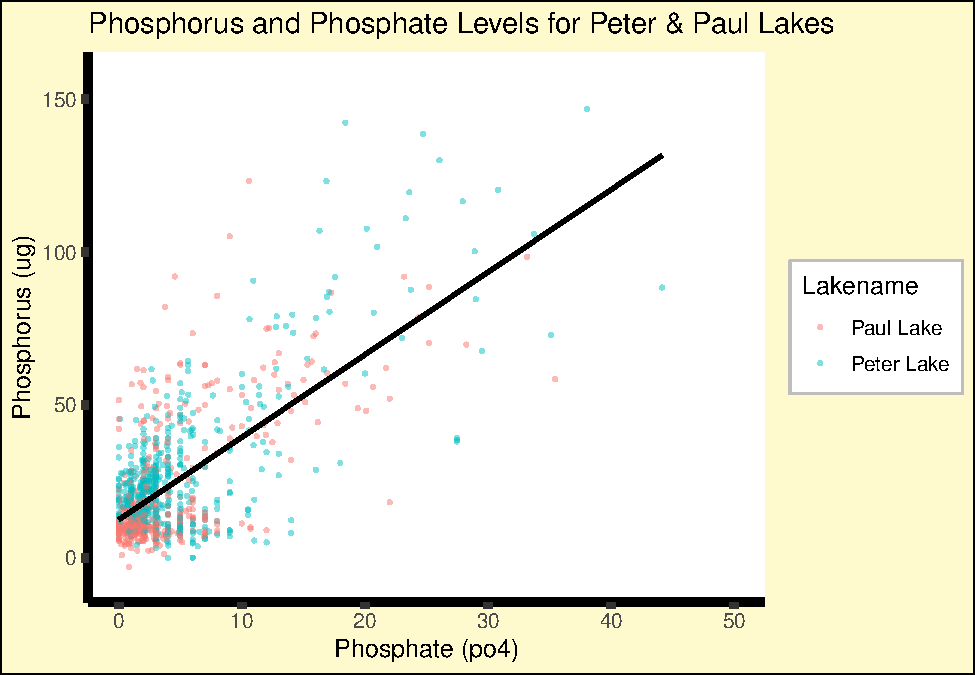
\includegraphics{EmmaChilds_A05_DataVisualization_files/figure-latex/plot total P vs PO4-1.pdf}

\begin{Shaded}
\begin{Highlighting}[]
\CommentTok{\#Plotted total phosphorus by phosphate and added best fit line. }
\end{Highlighting}
\end{Shaded}

\begin{enumerate}
\def\labelenumi{\arabic{enumi}.}
\setcounter{enumi}{4}
\tightlist
\item
  {[}NTL-LTER{]} Make three separate boxplots of (a) temperature, (b)
  TP, and (c) TN, with month as the x axis and lake as a color
  aesthetic. Then, create a cowplot that combines the three graphs. Make
  sure that only one legend is present and that graph axes are aligned.
\end{enumerate}

Tip: R has a build in variable called \texttt{month.abb} that returns a
list of months;see \url{https://r-lang.com/month-abb-in-r-with-example}

\begin{Shaded}
\begin{Highlighting}[]
\CommentTok{\#5 }
\CommentTok{\#Part a.}
\NormalTok{box\_temps }\OtherTok{\textless{}{-}}\NormalTok{ NTL.Chem.Nutrients.PeterPaul }\SpecialCharTok{\%\textgreater{}\%}
  \FunctionTok{ggplot}\NormalTok{(}
    \FunctionTok{aes}\NormalTok{(}\AttributeTok{x=}\FunctionTok{factor}\NormalTok{(month,}\AttributeTok{level=}\DecValTok{1}\SpecialCharTok{:}\DecValTok{12}\NormalTok{,}\AttributeTok{labels =}\NormalTok{ month.abb),}
      \AttributeTok{y=}\NormalTok{temperature\_C,}
      \AttributeTok{color=}\NormalTok{lakename)}
\NormalTok{  ) }\SpecialCharTok{+} 
  \FunctionTok{geom\_boxplot}\NormalTok{(}\AttributeTok{size=}\FloatTok{0.5}\NormalTok{, }\AttributeTok{alpha=}\FloatTok{0.5}\NormalTok{) }\SpecialCharTok{+}
    \FunctionTok{labs}\NormalTok{(}
      \AttributeTok{title =} \StringTok{"Temperatures for Peter \& Paul Lakes"}\NormalTok{,}
      \AttributeTok{x=}\StringTok{"Month"}\NormalTok{,}
      \AttributeTok{y=}\StringTok{"Temperature (C)"}\NormalTok{, }
      \AttributeTok{color=}\StringTok{"Lakename"}
\NormalTok{    ) }

\FunctionTok{print}\NormalTok{(box\_temps)}
\end{Highlighting}
\end{Shaded}

\begin{verbatim}
## Warning: Removed 3566 rows containing non-finite values (`stat_boxplot()`).
\end{verbatim}

\includegraphics{EmmaChilds_A05_DataVisualization_files/figure-latex/Create boxplots-1.pdf}

\begin{Shaded}
\begin{Highlighting}[]
\CommentTok{\#Part b.}
\NormalTok{box\_TP }\OtherTok{\textless{}{-}}\NormalTok{ NTL.Chem.Nutrients.PeterPaul }\SpecialCharTok{\%\textgreater{}\%}
  \FunctionTok{ggplot}\NormalTok{(}
    \FunctionTok{aes}\NormalTok{(}\AttributeTok{x=}\FunctionTok{factor}\NormalTok{(month,}\AttributeTok{level=}\DecValTok{1}\SpecialCharTok{:}\DecValTok{12}\NormalTok{,}\AttributeTok{labels =}\NormalTok{ month.abb),}
      \AttributeTok{y=}\NormalTok{tp\_ug,}
      \AttributeTok{color=}\NormalTok{lakename)}
\NormalTok{  ) }\SpecialCharTok{+} 
  \FunctionTok{geom\_boxplot}\NormalTok{(}\AttributeTok{size=}\FloatTok{0.5}\NormalTok{, }\AttributeTok{alpha=}\FloatTok{0.5}\NormalTok{) }\SpecialCharTok{+}
    \FunctionTok{labs}\NormalTok{(}
      \AttributeTok{title =} \StringTok{"Total Phosphorus for Peter \& Paul Lakes"}\NormalTok{,}
      \AttributeTok{x=}\StringTok{"Month"}\NormalTok{,}
      \AttributeTok{y=}\StringTok{"Total Phosphorus (ug)"}\NormalTok{, }
      \AttributeTok{color=}\StringTok{"Lakename"}
\NormalTok{    ) }

\FunctionTok{print}\NormalTok{(box\_TP)}
\end{Highlighting}
\end{Shaded}

\begin{verbatim}
## Warning: Removed 20729 rows containing non-finite values (`stat_boxplot()`).
\end{verbatim}

\includegraphics{EmmaChilds_A05_DataVisualization_files/figure-latex/Create boxplots-2.pdf}

\begin{Shaded}
\begin{Highlighting}[]
\CommentTok{\#Part c.}
\NormalTok{box\_TN }\OtherTok{\textless{}{-}}\NormalTok{ NTL.Chem.Nutrients.PeterPaul }\SpecialCharTok{\%\textgreater{}\%}
  \FunctionTok{ggplot}\NormalTok{(}
    \FunctionTok{aes}\NormalTok{(}\AttributeTok{x=}\FunctionTok{factor}\NormalTok{(month,}\AttributeTok{level=}\DecValTok{1}\SpecialCharTok{:}\DecValTok{12}\NormalTok{,}\AttributeTok{labels =}\NormalTok{ month.abb),}
      \AttributeTok{y=}\NormalTok{tn\_ug,}
      \AttributeTok{color=}\NormalTok{lakename)}
\NormalTok{  ) }\SpecialCharTok{+} 
  \FunctionTok{geom\_boxplot}\NormalTok{(}\AttributeTok{size=}\FloatTok{0.5}\NormalTok{, }\AttributeTok{alpha=}\FloatTok{0.5}\NormalTok{) }\SpecialCharTok{+}
    \FunctionTok{labs}\NormalTok{(}
      \AttributeTok{title =} \StringTok{"Total Nitrogen for Peter \& Paul Lakes"}\NormalTok{,}
      \AttributeTok{x=}\StringTok{"Month"}\NormalTok{,}
      \AttributeTok{y=}\StringTok{"Total Nitogren (ug)"}\NormalTok{, }
      \AttributeTok{color=}\StringTok{"Lakename"}
\NormalTok{    ) }

\FunctionTok{print}\NormalTok{(box\_TN)}
\end{Highlighting}
\end{Shaded}

\begin{verbatim}
## Warning: Removed 21583 rows containing non-finite values (`stat_boxplot()`).
\end{verbatim}

\includegraphics{EmmaChilds_A05_DataVisualization_files/figure-latex/Create boxplots-3.pdf}

\begin{Shaded}
\begin{Highlighting}[]
\CommentTok{\#Coded all three box plots and ran them successfully, I think!}

\CommentTok{\#Part d/cowplot.}
\CommentTok{\#install.packages("cowplot") {-} already done}
\FunctionTok{library}\NormalTok{(cowplot)}

\FunctionTok{plot\_grid}\NormalTok{(box\_temps, box\_TP, box\_TN, }\AttributeTok{labels =} \FunctionTok{c}\NormalTok{(}\StringTok{\textquotesingle{}Temperature (C)\textquotesingle{}}\NormalTok{, }\StringTok{\textquotesingle{}Total Phosporus\textquotesingle{}}\NormalTok{, }\StringTok{\textquotesingle{}Total Nitrogen\textquotesingle{}}\NormalTok{), }\AttributeTok{label\_size =} \DecValTok{12}\NormalTok{)}
\end{Highlighting}
\end{Shaded}

\begin{verbatim}
## Warning: Removed 3566 rows containing non-finite values (`stat_boxplot()`).
\end{verbatim}

\begin{verbatim}
## Warning: Removed 20729 rows containing non-finite values (`stat_boxplot()`).
\end{verbatim}

\begin{verbatim}
## Warning: Removed 21583 rows containing non-finite values (`stat_boxplot()`).
\end{verbatim}

\includegraphics{EmmaChilds_A05_DataVisualization_files/figure-latex/Create boxplots-4.pdf}

\begin{Shaded}
\begin{Highlighting}[]
\CommentTok{\#p1 \textless{}{-} ggplot(box\_temps, aes(x=month, y=temperature\_C)) + geom\_point()}
\CommentTok{\#p2 \textless{}{-} ggplot(box\_TP, aes(x=month, y=tp\_ug)) + geom\_point()}
\CommentTok{\#p3 \textless{}{-} ggplot(box\_TN, aes(x=month, y=tn\_ug)) + geom\_point()}
\CommentTok{\#This last section may not be correct, but I was playing around with different methods and tried this one. }
\end{Highlighting}
\end{Shaded}

Question: What do you observe about the variables of interest over
seasons and between lakes?

\begin{quote}
Answer: It is a little difficult to say from just looking at the graphs,
but it seems like the temperatures are relatively similar between lakes.
Peter Lake seems to have higher phosphorus, with highest values in the
summer months, and pretty similar with total nitrogen as well in
comparison to Paul Lake.
\end{quote}

\begin{enumerate}
\def\labelenumi{\arabic{enumi}.}
\setcounter{enumi}{5}
\item
  {[}Niwot Ridge{]} Plot a subset of the litter dataset by displaying
  only the ``Needles'' functional group. Plot the dry mass of needle
  litter by date and separate by NLCD class with a color aesthetic. (no
  need to adjust the name of each land use)
\item
  {[}Niwot Ridge{]} Now, plot the same plot but with NLCD classes
  separated into three facets rather than separated by color.
\end{enumerate}

\begin{Shaded}
\begin{Highlighting}[]
\CommentTok{\#6}
\CommentTok{\#Plotting "Needles" functional group by date and separating with color}
\NormalTok{litter\_subset }\OtherTok{\textless{}{-}}\NormalTok{ NEON.litter }\SpecialCharTok{\%\textgreater{}\%} 
  \FunctionTok{filter}\NormalTok{(functionalGroup}\SpecialCharTok{==}\StringTok{\textquotesingle{}Needles\textquotesingle{}}\NormalTok{) }\SpecialCharTok{\%\textgreater{}\%} 
  \FunctionTok{ggplot}\NormalTok{(}\FunctionTok{aes}\NormalTok{(}
      \AttributeTok{x=}\NormalTok{collectDate,}
      \AttributeTok{y=}\NormalTok{dryMass,}
      \AttributeTok{color=}\NormalTok{nlcdClass)}
\NormalTok{    ) }\SpecialCharTok{+} 
  \FunctionTok{geom\_point}\NormalTok{(}\AttributeTok{size=}\FloatTok{0.5}\NormalTok{,}\AttributeTok{alpha=}\FloatTok{0.5}\NormalTok{) }\SpecialCharTok{+}
    \FunctionTok{labs}\NormalTok{(}
    \AttributeTok{title=}\StringTok{"Dry Mass of Needle Litter"}\NormalTok{,}
    \AttributeTok{x=}\StringTok{"Date"}\NormalTok{,}
    \AttributeTok{y=}\StringTok{"Dry Mass"}\NormalTok{,}
    \AttributeTok{color=}\StringTok{"NLCD Class"}
\NormalTok{    )}

\FunctionTok{print}\NormalTok{(litter\_subset)}
\end{Highlighting}
\end{Shaded}

\includegraphics{EmmaChilds_A05_DataVisualization_files/figure-latex/Plot litter-1.pdf}

\begin{Shaded}
\begin{Highlighting}[]
\CommentTok{\#7}
\CommentTok{\#Plotting dry mass again, but faceted by NLCD class}
\NormalTok{litter.subset.faceted }\OtherTok{\textless{}{-}}\NormalTok{ NEON.litter }\SpecialCharTok{\%\textgreater{}\%}
  \FunctionTok{filter}\NormalTok{(functionalGroup}\SpecialCharTok{==}\StringTok{\textquotesingle{}Needles\textquotesingle{}}\NormalTok{) }\SpecialCharTok{\%\textgreater{}\%} 
  \FunctionTok{ggplot}\NormalTok{(}
     \FunctionTok{aes}\NormalTok{(}\AttributeTok{x=}\NormalTok{collectDate, }
         \AttributeTok{y=}\NormalTok{dryMass,)) }\SpecialCharTok{+}
  \FunctionTok{geom\_point}\NormalTok{(}\AttributeTok{size=}\FloatTok{0.5}\NormalTok{,}\AttributeTok{alpha=}\FloatTok{0.5}\NormalTok{) }\SpecialCharTok{+}
  \FunctionTok{facet\_wrap}\NormalTok{(}\FunctionTok{vars}\NormalTok{(nlcdClass)) }\SpecialCharTok{+}
    \FunctionTok{labs}\NormalTok{(}
    \AttributeTok{title=}\StringTok{"Dry Mass of Needle Litter"}\NormalTok{,}
    \AttributeTok{x=}\StringTok{"Date"}\NormalTok{,}
    \AttributeTok{y=}\StringTok{"Dry Mass"}
\NormalTok{    )}

\FunctionTok{print}\NormalTok{(litter.subset.faceted)}
\end{Highlighting}
\end{Shaded}

\includegraphics{EmmaChilds_A05_DataVisualization_files/figure-latex/Plot litter-2.pdf}
Question: Which of these plots (6 vs.~7) do you think is more effective,
and why?

\begin{quote}
Answer: I find number 6 more effective because I think having all the
data on one graph with different colors allows for better comparision
between NLCD classes than three separate graphs.
\end{quote}

\end{document}
